\documentclass[10pt]{article}
%Spaces etc
\usepackage{setspace}

% Headers
\usepackage[hidelinks]{hyperref}
\usepackage[utf8]{inputenc}

\usepackage{fancyhdr}

\usepackage{graphicx}
\usepackage{float}

\usepackage{cleveref}

% BibTex
\usepackage[backend=biber]{biblatex}
\DeclareLanguageMapping{american}{american-apa}
\addbibresource{sources.bib}

% The page headers
\pagestyle{fancy}
\fancyhf{}
\lhead{ \fancyplain{}{Let The DNA Speak} }
\rhead{ \fancyplain{}{\thepage} }

\title{Let The DNA Speak\\Final Report}

\author{Stefan Appelhoff, Kim Philipp Jablonski, Nina Krüger, Sourabh Lal, Tom Wiesing \& Mengyuan Zhang}

\begin{document}

\begin{titlepage}
\thispagestyle{empty}
\begin{center}

\textsc{\huge Let the DNA speak}\\[2cm]
\textsc{\Huge Final Report}\\[6cm]

\Large{Jacobs University Bremen\\
Spring Semester 2014\\020077 USC - Let the Data Speak}
\vspace*{1.2cm}

\Large{Instructors:\\Dr. Aidan Boyle\\Prof. Dr. Adalbert F.X. Wilhelm}
\vspace*{1.2cm}

\Large{Authors:\\Stefan Appelhoff, Kim Philipp Jablonski, \\Nina Krüger, Sourabh Lal, Tom Wiesing \& Mengyuan Zhang}
\vspace*{1.2cm}

\end{center}

\end{titlepage}


\clearpage
\thispagestyle{empty}
\tableofcontents
\newpage

\setcounter{page}{1}
\section{Introduction}
Let the DNA Speak is an application that can be used for the sonification of DNA 
codes for the purpose of comparison. It has been developed as part of the course "Let the Data 
Speak" at Jacobs University Bremen. There have been various techniques used in the past to 
compare DNA. Ranging from graphical devices like chromatograms, over more data centered 
possibilities like simple tables, they offer a wide variety of learning and perceiving the 
structure of DNA through many different senses. However, this application addresses an often 
neglected technique; sonification. This report is a documentation of the development and 
usage for this application. The application itself can be accessed via \url{http://letthednaspeak.tk/}, while the source code can be found at \url{https://github.com/kpj/LetTheDnaSpeak}.

\section{Statistics}
\subsection{Sources of Data}
In our datasets, we are dealing with string data containing 4 different letters, which 
stand for the fundamental nucleo-bases making up every DNA: Adenine (A), Cytosine (C), 
Guanine (G), and Thymine (T). These bases are biologically organized in triplets, 
representing amino acids which finally make up proteins, the building blocks of our life (\cref{figure:codon_sun}).

\begin{figure}[H]
  \centering

  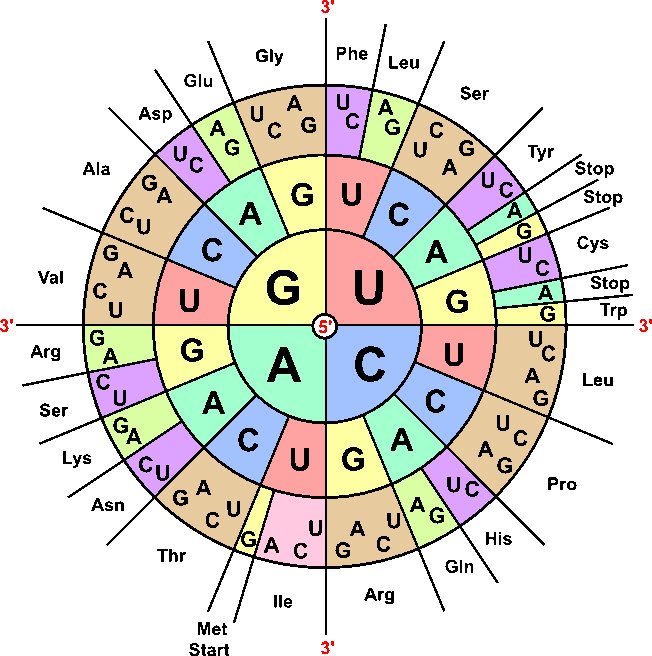
\includegraphics[width=8cm]{codon_sun.png}
  
  \caption{Codon Sun specifying which base combinations make up which amino acids \cite{codonSun}}
  \label{figure:codon_sun}
\end{figure}

As 
an example, one could look at the DNA sequences of hemoglobin, a protein which is 
responsible for the oxygen transport in the blood of all vertebrates. When affected by a 
disease such as the Sickle Cell Disease (SCD), the Hemoglobin gene is mutated and thus, the 
string of triplets deviates from a normal Hemoglobin gene.


\begin{center}
  \emph{Sequence for Normal Hemoglobin}\\
  ATG GTG CAC CTG ACT CCT \textbf{GAG} GAG AAG TCT GCC GTT ACT\\
  \medskip
  \emph{Sequence for Sickle Cell Hemoglobin}\\
  ATG GTG CAC CTG ACT CCT \textbf{GTG} GAG AAG TCT GCC GTT ACT\\
\end{center}

The difference between the two DNA strings is almost unnoticeable (one base in the 
seventh triplet deviates in the mutated gene). However, this difference causes SCD and 
ultimately leads to symptoms such as a shorter life span \cite{more_sickles} and interestingly 
resistance against the infectious disease Malaria \cite{sickle_cells}.
\subsection{Importance of this Type of Data}
There are several areas of application for our project. We see its main benefits in education. 
Our sonification demonstrates in an impressive way how small the difference between a 
healthy human being and one with a disease can be, as in the case of sickle cell anaemia. 
Here, due to a point mutation only one base is changed, which results in only one different 
note in our sonification. On the other hand, Treacher Collins Syndrome for example shifts the 
whole reading frame of the DNA by deleting two bases, which then results in a completely 
different tune; the defect is clearly audible. Those examples can be an impressive way to 
teach children about different kinds of mutations. Furthermore the sonification might be 
helpful for professionals to detect mutations in DNA strands. As it could be seen for deletion 
mutations a disease can result from only one changed base. Those small differences are 
almost impossible to identify reliably with visual search. With the approach of sonification 
we wanted to show, that mapping the DNA strands to auditory dimensions can facilitate the 
detection of such small yet crucial differences in DNA strands, as a change in the reading 
frame will suddenly result in a completely different sonification. 
\subsection{Data Features of Specific Interest}
For our sonification, the most interesting data features are of course deviations in 
bases when two different DNA strands are being compared. However, there are several other 
aspects, which become apparent in our sonification such as measures of central tendency. 
E.g., the frequency that occurs most often throughout the sonification represents the amino acid with the highest mode in the DNA strand. Also measures of statistical dispersion such as 
the variance are represented by the sonification in that e.g., a sound that is playing a broad 
range of frequencies quickly changing in time signifies a large variance.
\subsection{Aim of Sonification}
There are two things we are trying to sonify. First is the structure and patterns in the 
DNA, such as repetition, symmetry, correlations and general distributions. The second is the 
differences between different strands of DNAs. 

\section{Sonification}
\subsection{Mapping imposed on the Listener}
For our project, no fixed mapping is imposed on the listener. Instead, we offer a 
“sonification-tool”: Each user can choose their own mapping from a selection and experiment 
with it. We provide a number of pre selections concerning how DNA strands are mapped to 
musical dimensions (described in detail below) — additionally we offer the option to choose 
from a list of instruments, to sonify the data. With these possibilities, we think that any user 
of our sonification-tool can try subjectively, which mapping is appropriate for the current 
needs. As our tool mainly aims at the comparison of two different DNA strands played at the 
same time, it is of particular importance to be able to chose an instrument independently for 
each of the two strands. Having two diverging timbres (e.g., Piano versus Marimba) will help 
the listener to distinguish the two DNA strands and therefore notice differences more easily.
\subsection{Details of the Mapping}
Our sonification currently offers three different modes of transforming base sequences 
into music. The first one uses a distinct mapping from three bases to one note by encoding a nucleotide as a number $n \in \{0,1,2,3\}$ grouping them in clusters of three, interpreting 
them as an integer in base 4 and converting them into the decimal system. The last step also 
includes a bijective mapping to the range $21$, $121$, as that 
represents the spectrum of common MIDI instruments. This allows to observe any pattern in 
the DNA without any normalization with respect to biological patterns.
These biological patterns however, play a big role in our life. This is the reason why we 
created another parser, which starts with mapping base triplets to their respective amino acids 
using the common scheme of a codon sun. This allows the user to examine 
patterns which are more closely related to the actual biological composition of the sequence.
In our last step, we tried to improve the musical representation of the provided DNA strands 
by introducing a combination of notes played at the same time together with two different 
tone scales (i.e. C-major and pentatonic). The aforementioned combination was realised by 
playing the actual notes simultaneously with fifths which are determined by every 8th note 
occurring in the strand.
\subsection{Aiming for a particular Aesthetic}
Some DNA strands can be very long and therefore a user would not want to be 
exposed to disturbing sounds for a large timespan. For our tool it is thus important to have a 
“listenable” output with the custom sonification. Aesthetically, we aim for a meditative sound 
with a stable speed and only one mapped instrument per DNA strand. This meditative sound 
is disrupted as soon as the two DNA strands show differences. At such a moment, the notes 
played together will also be different and in the most cases, this difference will be noticeable. 
Overall, a user will be able to concentrate easily on the sonification — getting completely 
drawn into the flow and being kicked out of the flow, as soon as a difference in DNA strands 
appears.

\section{Meaning}
\subsection{Possible Extractions from the Data}
The listener will easily pick up the melodic difference in the music and thus be aware 
of the differences in the base triplets. In particular, some minor changes in the bases may 
cause the existence/non-existence of certain proteins thus can be crucial to the being - and in 
some cases it is a life-or-death situation. The minor differences in the DNA will be amplified 
and artistified through music to match their significance and for the listener to appreciate.
\subsection{Learning Curve for Trained Listeners}
The learning curve is easy, any listener will appreciate the difference in different DNA 
strands. However, the learning curve also very much depends on the familiarity with music 
and the purpose of using the sonification. As for our example of hemoglobin, a point mutation 
might be barely audible for inexperienced listeners. Thus, by repetitive usage, the listener 
might train to also detect such minor changes in the tune.

\section{Conclusion}
Our project offers a tool with a magnitude of different options allowing the user to 
experiment with their data. This variety allows them to adjust our product to their individual 
needs. In particular, it allows the analysis of DNA strands for people, who (for whatever 
reason) cannot rely on textual representations.

\newpage
\clearpage
\pagestyle{empty}

\nocite{*}
\doublespacing
\printbibliography

\end{document}